
\section{Empirical Evaluation}

\remark{Start this section with the experimental rationale... what
  hypotheses are we trying to evaluate in this section?}

\subsection{Networks}

Three networks of increasing complexity were defined for performance
analysis and comparison. The first consists of a two-way avenue with
three traffic light controlled intersections with 3 one-way side
streets, as shown in figure \ref{fig:network3}. The second is an
extension of the first to include a second parallel two-way avenue and
an additional 3 traffic lights to control the side streets, as shown
in figure \ref{fig:network6}. And the third is a grid of three EW
two-way avenues, with two NS two-way avenues and one NS one way street
and a NE to SW diagonal one-way street, as shown in figure
\ref{fig:network9}.

The traversal time of each queue in all three networks is set at 9
seconds (a distance of about 100m with a free flow speed of
50km/h). The maximum capacity of each queue is set at 60 cars. Flows
are defined only straight ahead from the head of each queue into the
tail of the next - there is no turning traffic, and in all cases the
maximum flow rate is set at 5 cars per second. Each traffic light has
two phases - NS and EW. The minimum phase time is 1 second and the
maximum phase time is 3 seconds. The minimum cycle time of both the
phases is 2 seconds and the maximum is 6.

For each network a background level of flow is first established and
then later increased as a wave of higher volume traffic is injected
into the network at some of the streets. Then all the traffic is
allowed to clear the network before ending the simulation to support
an analysis of the total travel time in the network. The details of
the flow levels is given in tables \ref{tab:net1wave},
\ref{tab:net2wave} and \ref{tab:net3wave}.

\subsection{Experimental Methodology}

With a CTM based model the $\DT[]$ must remain fixed through out the
optimisation period, while the QTM supports non-homogeneous time steps
mixed with homogeneous time steps. To exploit this we define a
mutli-step solver that allows the time step of the plan to increase
overtime. Such an increase will reduce the total number of variables
for the same optimisation period compared to a homogeneous plan, with
the trade off that the plan will be have less resolution over
time. But this seems acceptable as the accuracy of the plan will also
decrease overtime the further from the initial conditions.

We start by generating a plan for a longer horizon using an increasing
time step so that the solver has greater visibility of the impact of
an earlier planning decision across a larger part of the network for
the same number of variables as a fixed time step. We then keep the
first part of this plan where the accuracy is highest and discard the
rest, where the time steps where larger. Once the retained section of
plan has be carried out, we generate another long horizon plan and
repeat (see figure \ref{fig:multiplan}.

We call the long term plan a major frame and the shorter section of a
major frame that we retain, a minor frame. We use a minor frame of 10
seconds and increasing major frame sizes from 20 upwards and generate
such mutlistep plans with both a homogeneous $\DT[]$ of 0.25 seconds
and a non-homogenous $\DT[]$ ranging from fixed 0.25 second increments
during the minor frame and the increasing linearly until 1 second at
the horizon. We generated plans for all three networks using both the
homogeneous $\DT[]$ major frames and the non-homogeneous $\DT[]$ major
frames. For reference we also performed a full optimal solve using a
fixed $\DT[]$ of 0.25 seconds. Once we have generated a set of minor
frames, we combined them into a large fixed plan and simulate the flow
of in the network with a fixed $\DT[]$ of 0.25, to support a fair
comparison.

\begin{figure*}[t!]
\centering
%  trim={<left> <lower> <right> <upper>}
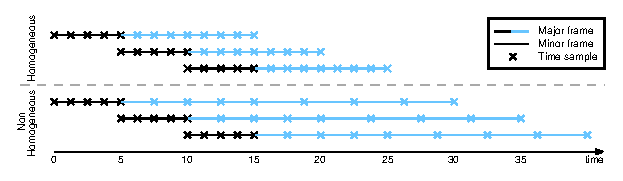
\includegraphics[width=1.0\textwidth]{non_homogeneous_control.eps}
\caption{Multi-step planning}
\label{fig:multiplan}
\end{figure*}


\begin{figure*}[t!]
\centering
%  trim={<left> <lower> <right> <upper>}
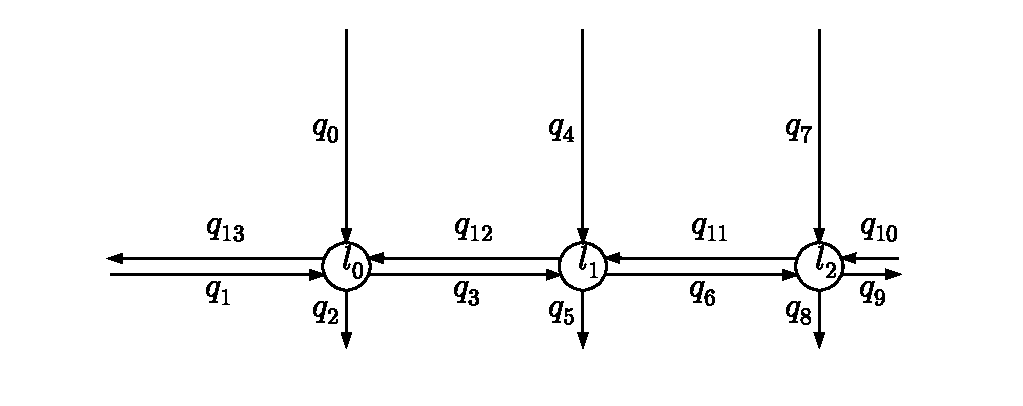
\includegraphics[width=0.75\textwidth]{network_3_lights}
\caption{Network 1}
\label{fig:network3}
\end{figure*}

\begin{table}[h]
\caption{Network 1 traffic parameters}
\label{tab:net1wave}
\centering
\begin{tabular}{cccccc}
\toprule
Queue & Background & End & Wave & Start &End\\ 
\midrule
$q_0$ & 1 & 85 & 1 & 55 & 70\\
$q_1$ & 2 & 85 & 4 & 55 & 70\\
$q_4$ & 4 & 85 & 4 & 55 & 70\\
$q_7$ & 4 & 85 & 4 & 55 & 70\\
$q_{10}$ & 2 & 85 & 4 & 55 & 70\\
\bottomrule\\
\end{tabular}
\end{table}


\begin{figure*}[t!]
\centering
%  trim={<left> <lower> <right> <upper>}
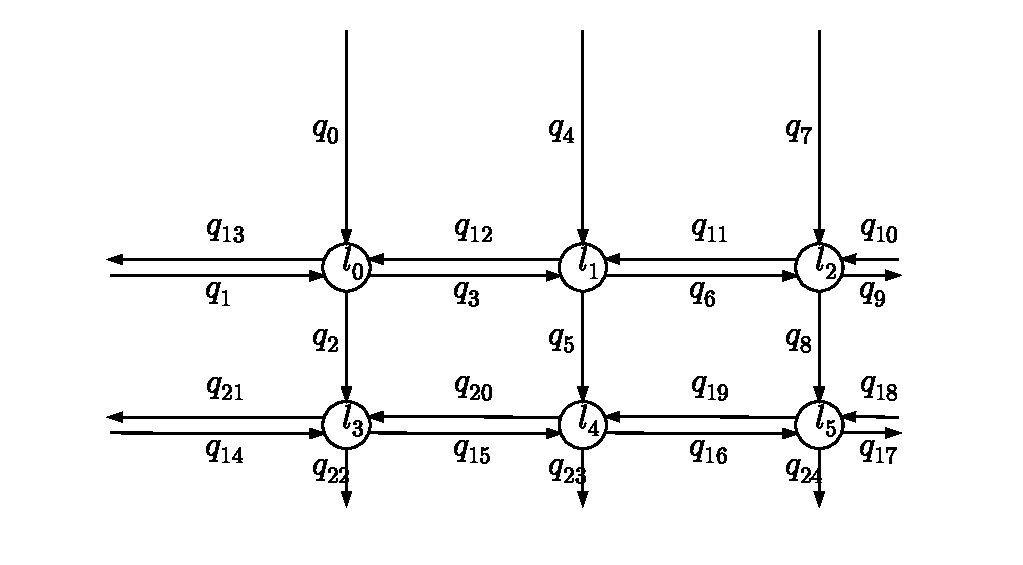
\includegraphics[width=0.75\textwidth]{network_6_lights}
\caption{Network 2}
\label{fig:network6}
\end{figure*}

\begin{table}[h]
\caption{Network 2 traffic parameters}
\label{tab:net2wave}
\centering
\begin{tabular}{cccccc}
\toprule
Queue & Background & End & Wave & Start &End\\ 
\midrule
$q_0$ & 1 & 85 & 1 & 55 & 70\\
$q_1$ & 2 & 85 & 4 & 55 & 70\\
$q_4$ & 4 & 85 & 4 & 55 & 70\\
$q_7$ & 4 & 85 & 4 & 55 & 70\\
$q_{10}$ & 2 & 85 & 4 & 55 & 70\\
$q_{14}$ & 4 & 85 & 4 & 55 & 70\\
$q_{18}$ & 2 & 85 & 4 & 55 & 70\\
\bottomrule\\
\end{tabular}
\end{table}


\begin{figure*}[t!]
\centering
%  trim={<left> <lower> <right> <upper>}
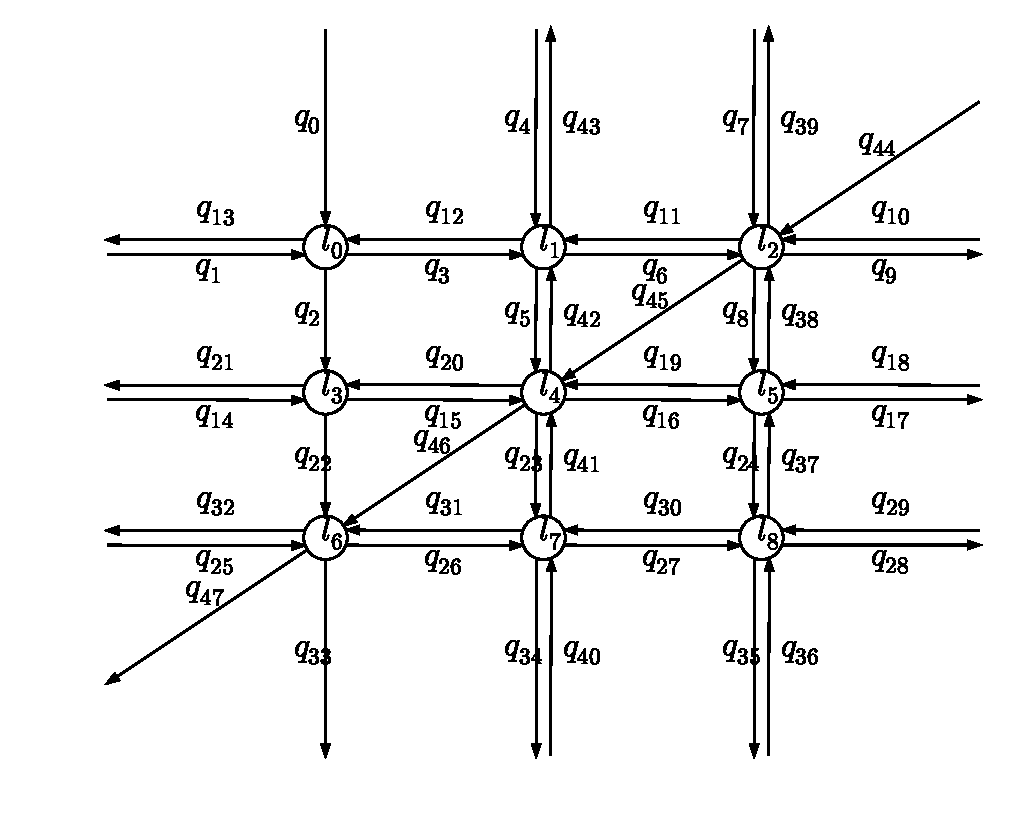
\includegraphics[width=0.75\textwidth]{network_9_lights}
\caption{Network 3}
\label{fig:network9}
\end{figure*}


\begin{table}[h]
\caption{Network 3 traffic parameters}
\label{tab:net3wave}
\centering
\begin{tabular}{cccccc}
\toprule
Queue & Background & End & Wave & Start &End\\ 
\midrule
$q_0$ & 1 & 85 & 1 & 55 & 70\\
$q_1$ & 2 & 85 & 4 & 55 & 70\\
$q_4$ & 4 & 85 & 4 & 55 & 70\\
$q_7$ & 4 & 85 & 4 & 55 & 70\\
$q_{10}$ & 2 & 85 & 4 & 55 & 70\\
$q_{14}$ & 4 & 85 & 4 & 55 & 70\\
$q_{18}$ & 2 & 85 & 4 & 55 & 70\\
$q_{25}$ & 4 & 85 & 4 & 55 & 70\\
$q_{29}$ & 2 & 85 & 4 & 55 & 70\\
$q_{36}$ & 2 & 85 & 4 & 55 & 70\\
$q_{40}$ & 2 & 85 & 4 & 55 & 70\\
$q_{44}$ & 2 & 85 & 4 & 55 & 70\\
\bottomrule\\
\end{tabular}
\end{table}

\subsection{Results}

We compared the performance of non-homogeneous and homogeneous $\DT[]$ in two ways: comparing the decrease in total travel time with increasing major frame size. And analysing the distribution of delay in each queue of the network. Figure \ref{fig:results} (a), (c) and (e) show a comparison between the number of time samples used in the major frame vs the \% improvement in total travel time. It can be seen that using a non homogenous $\DT[]$ converges towards the optimum more quickly than the homogeneous $\DT[]$ for the same number of time samples. Figure \ref{fig:results} (b), (d) and (f) show a comparison of distribution of delay across the network. This gives us an indication of the quality of the solution in terms of the number of vehicles that experience significant delay and if the plan may be starving some parts of the network.  The plots show three comparisons: at the point where the non-homogeneous $\DT[]$ first converges on the optimum solution, where the homogeneous $\DT[]$ first converges on the optimum solution, and the optimum solution. With all three networks the quality of the solutions improves or stays the same using an non-homogeneous $\DT[]$ compared to a homogeneous $\DT[]$.
Finally, figure \ref{fig:cumu} shows the how cumulative arrival and departure curves and the delay develop over time for $q_1$ of network 2. Figure \ref{fig:cumu} (a) shows the comparison at the point where the non-homogeneous $\DT[]$ first converges and shows that with the longer major frame of the non-homogeneous $\DT[]$, it is able to adopt a better signal plan early on to anticipate the wave of traffic that arrives at about the 55 second point, while the homogeneous $\DT[]$ with its shorter major frame initially prioritises the side street ($q_0$, $q_2$, $q_{22}$) over $q_1$ resulting in significant delay once the wave of traffic arrives. Once homogeneous $\DT[]$ has converged in Figure \ref{fig:cumu} (b), both plans are close to the optimum shown in Figure \ref{fig:cumu} (c).

\begin{figure*}[t!]
\centering

%  trim={<left> <lower> <right> <upper>}
\subfigure[]{
\label{subfig:travel_time_3}
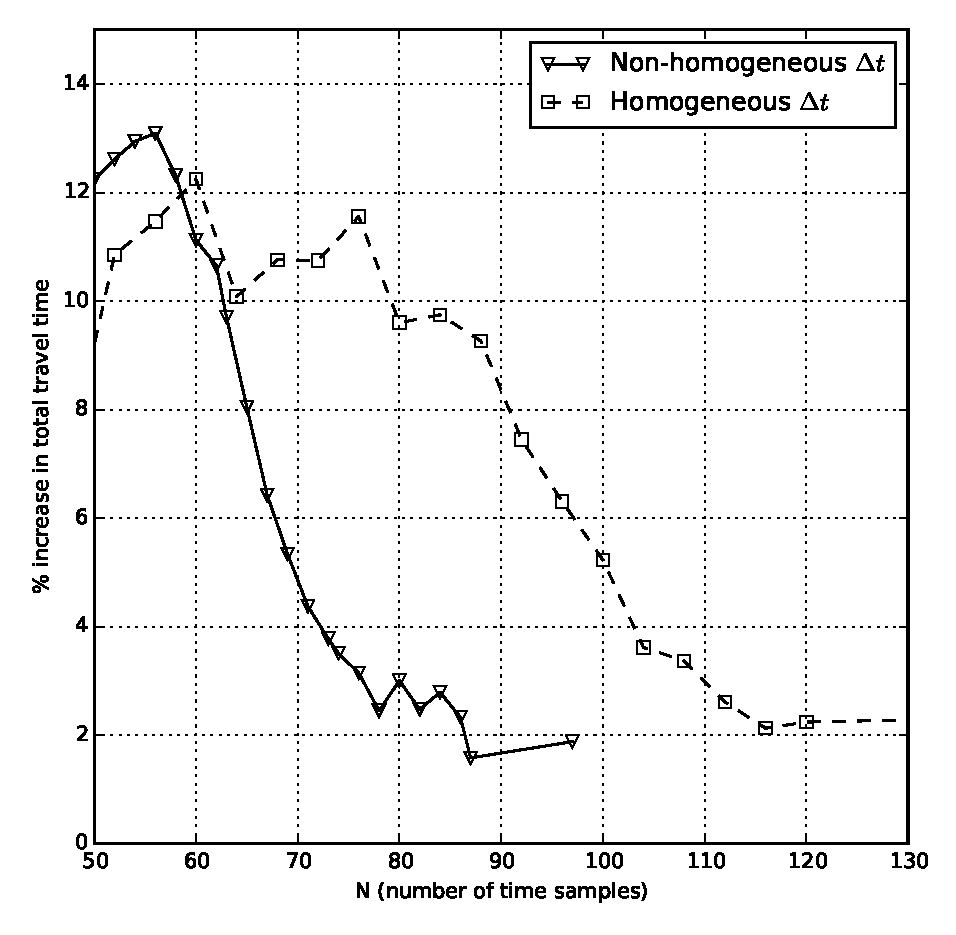
\includegraphics[width=0.4\textwidth]{samples_plot_3_lights}}
\subfigure[]{
\label{subfig:delay_3}
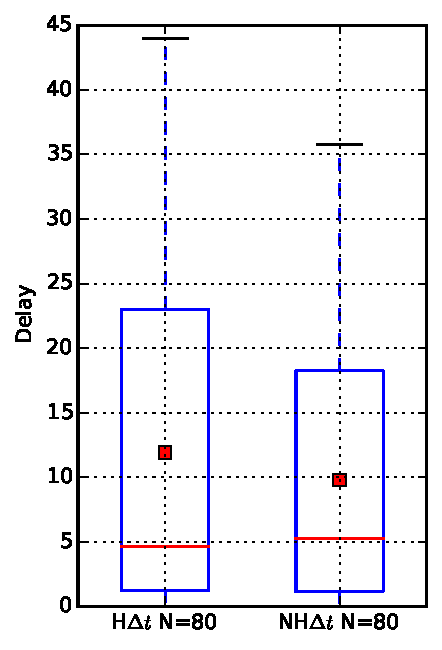
\includegraphics[keepaspectratio,height=0.3\textwidth]{box_plot_early_3l.pdf}
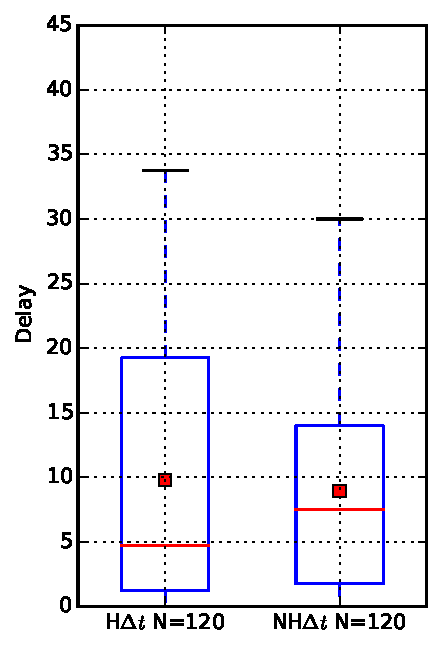
\includegraphics[keepaspectratio,height=0.3\textwidth]{box_plot_converg_3l.pdf}
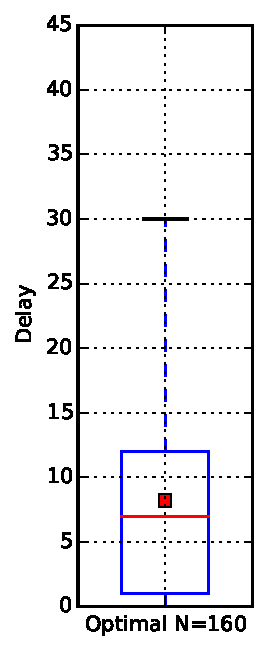
\includegraphics[keepaspectratio,height=0.3\textwidth]{box_plot_final_3l.pdf}}

\subfigure[]{
\label{subfig:travel_time_6}
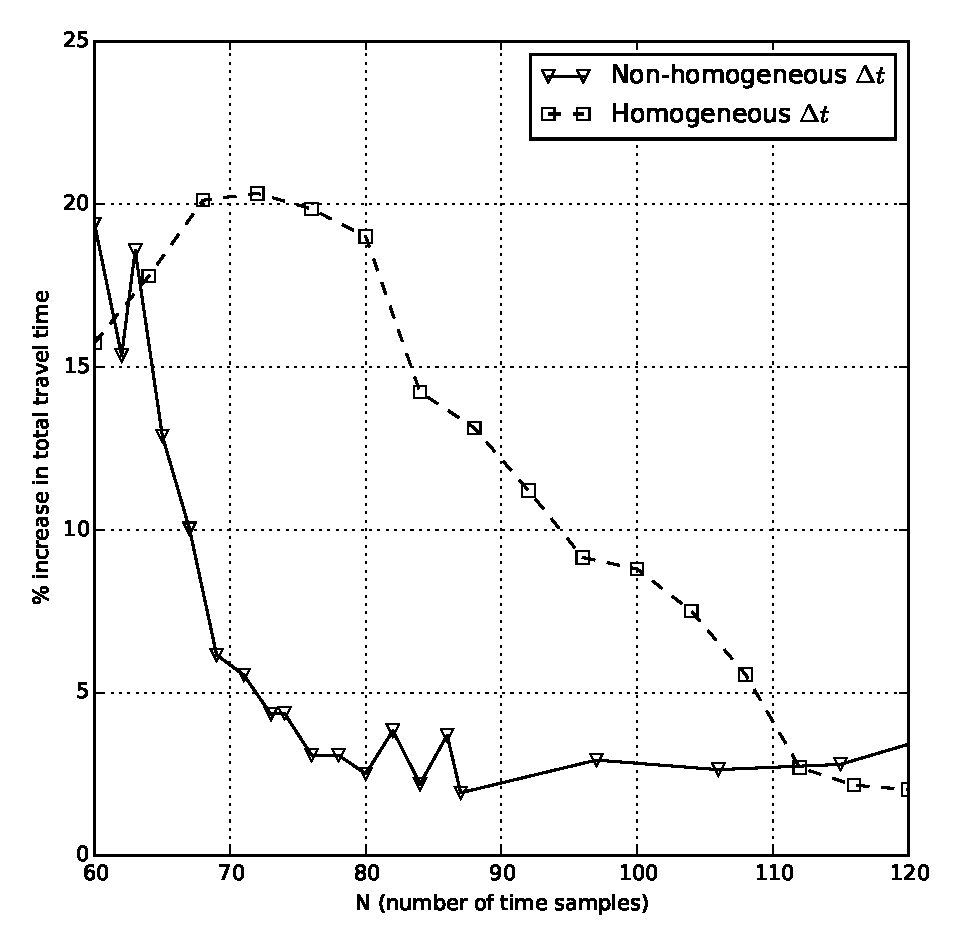
\includegraphics[width=0.4\textwidth]{samples_plot_6_lights}}
\subfigure[]{
\label{subfig:delay_6}
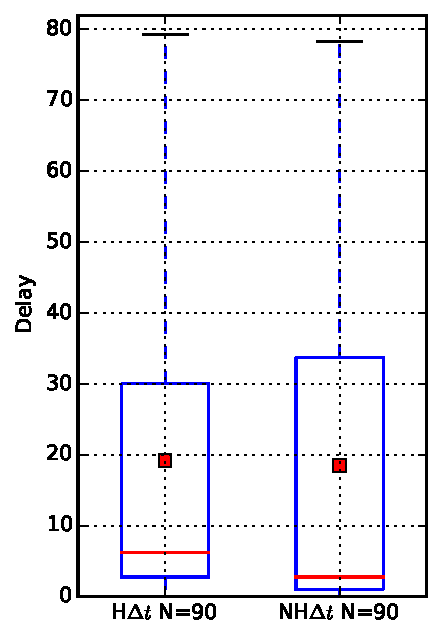
\includegraphics[keepaspectratio,height=0.3\textwidth]{box_plot_early_6l.pdf}
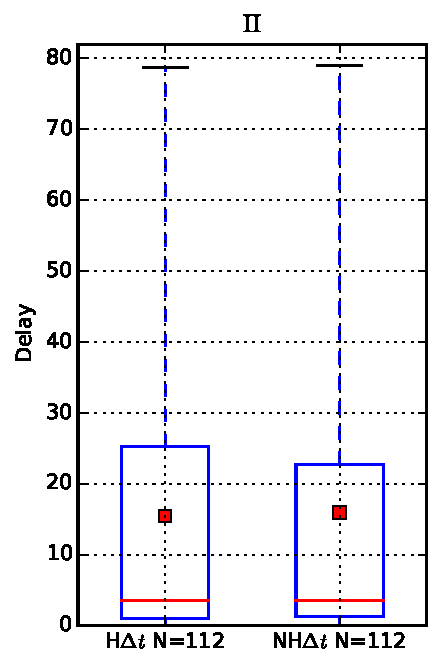
\includegraphics[keepaspectratio,height=0.3\textwidth]{box_plot_converg_6l.pdf}
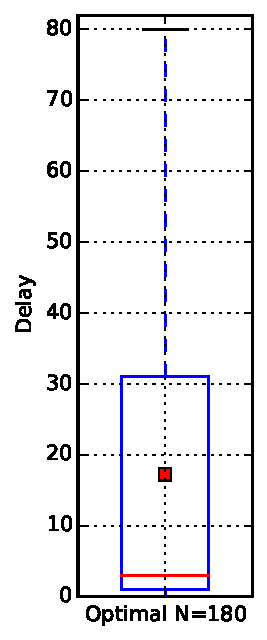
\includegraphics[keepaspectratio,height=0.3\textwidth]{box_plot_final_6l.pdf}}

\subfigure[]{
\label{subfig:travel_time_9}
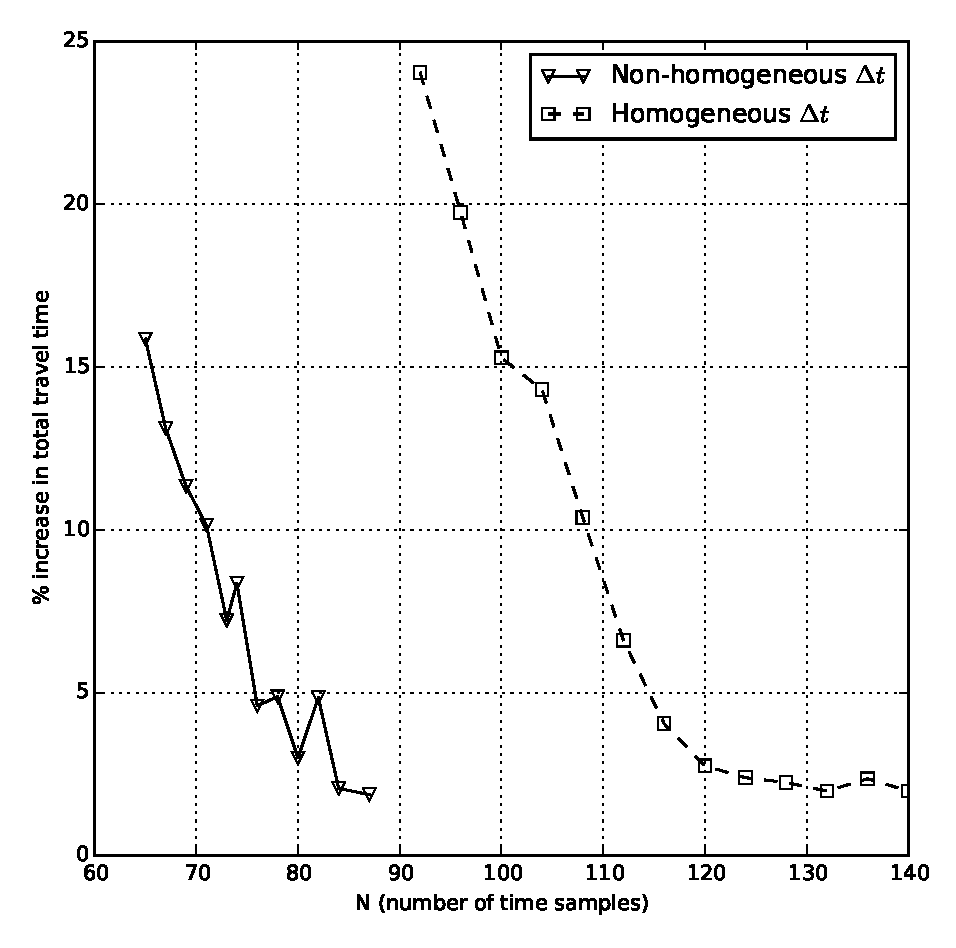
\includegraphics[width=0.4\textwidth]{samples_plot_9_lights}}
\subfigure[]{
\label{subfig:delay_9}
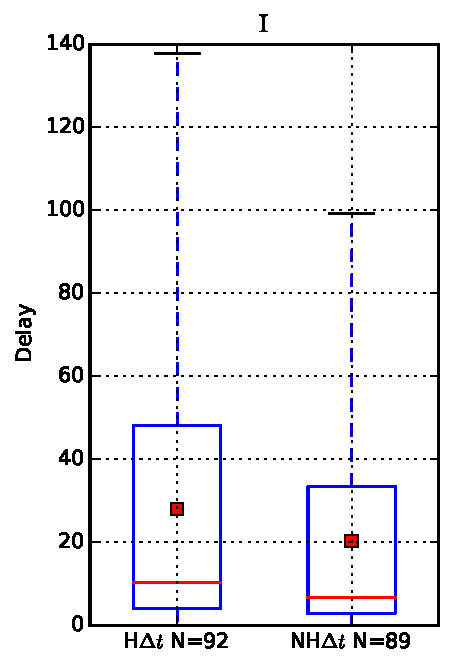
\includegraphics[keepaspectratio,height=0.3\textwidth]{box_plot_early_9l.pdf}
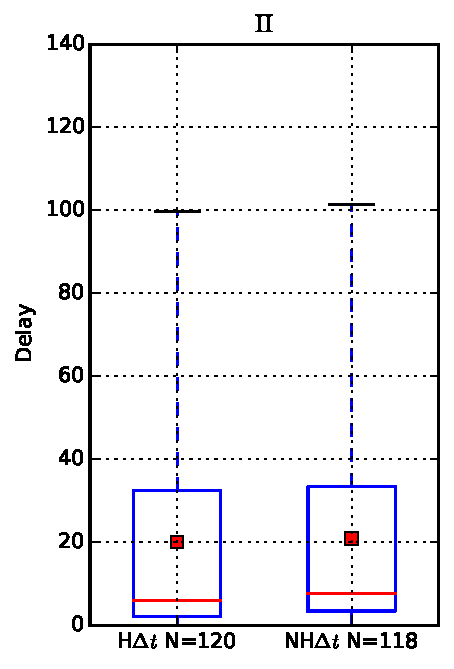
\includegraphics[keepaspectratio,height=0.3\textwidth]{box_plot_converg_9l.pdf}
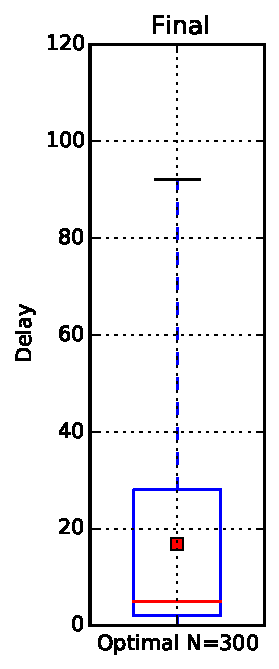
\includegraphics[keepaspectratio,height=0.3\textwidth]{box_plot_final_9l.pdf}}
\caption{Results for the three networks showing the comparitive \% improvement in total travel time for the network between using a homogeneous $\DT[]$ and a non-homogeneous $\DT[]$, and the distribution of delay time at the convergence point of non-homogeneous $\DT[]$, the convergence point of homogeneous $\DT[]$ and for the fully solved optimal solution. (a) and (b) 3 light avenue, (c) and (d) 6 light grid, and (e) and (f) 9 light grid,}
\label{fig:results}
\end{figure*}

\begin{figure*}[t!]
\centering

%  trim={<left> <lower> <right> <upper>}
\subfigure[]{
\label{subfig:cumu1}
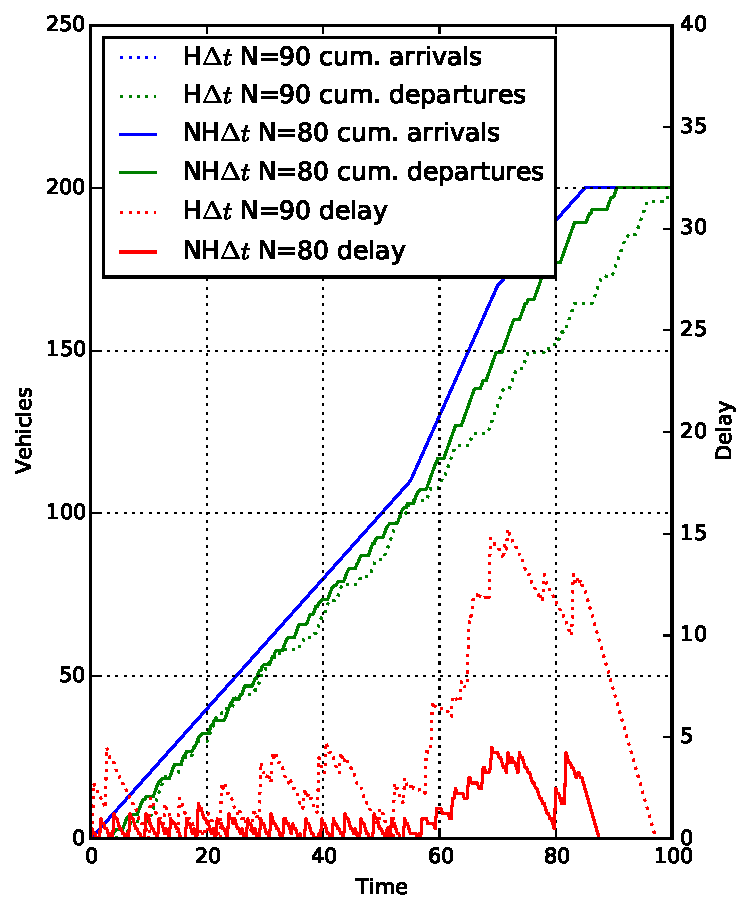
\includegraphics[width=0.32\textwidth]{cum_plot_early_6l.pdf}}
\subfigure[]{
\label{subfig:cumu2}
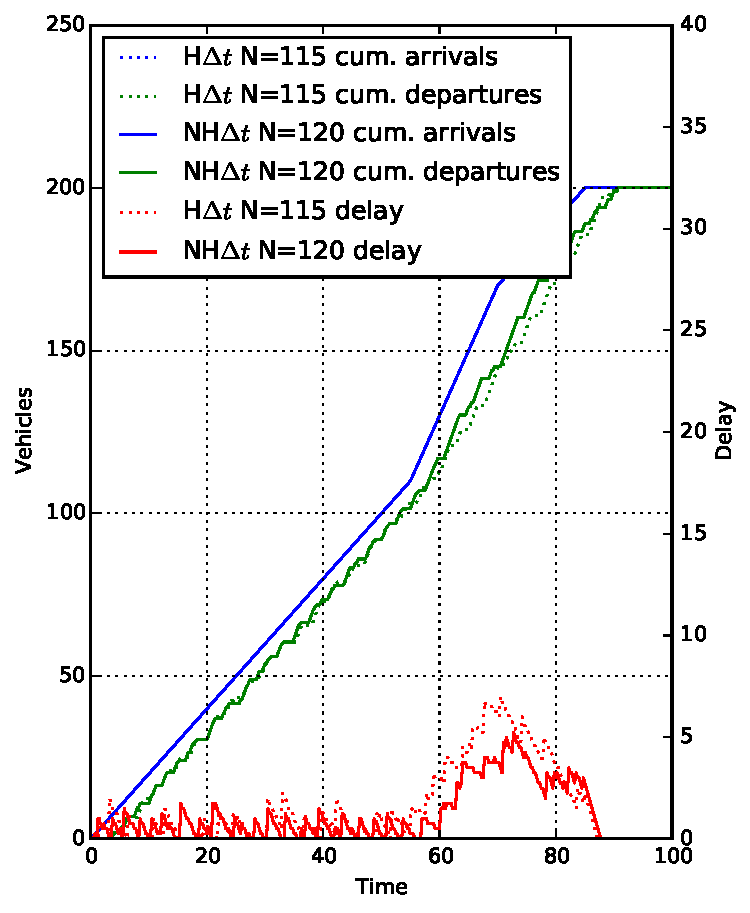
\includegraphics[width=0.32\textwidth]{cum_plot_converg_6l.pdf}}
\subfigure[]{
\label{subfig:cumu3}
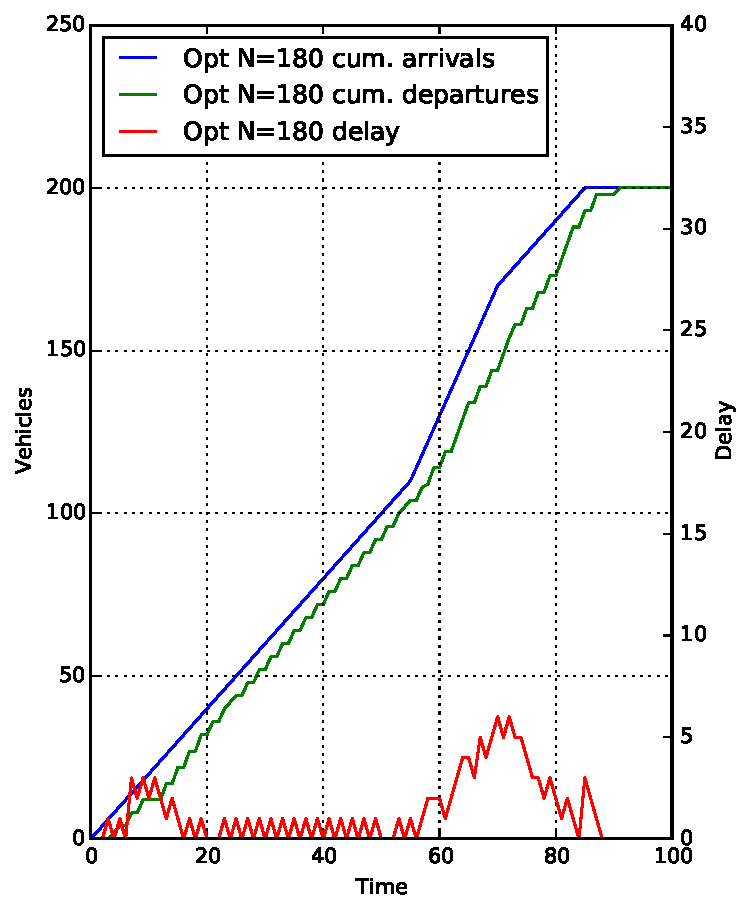
\includegraphics[width=0.32\textwidth]{cum_plot_final_6l.pdf}}
%\includegraphics[width=0.25\textwidth,trim={3cm 1.5cm 3cm 2.3cm},clip]{Satellite_Augmentation/test_17.eps}}
\caption{Cumulative arrival and departure curves and delay for queue 1 in the 6 light grid. (a) at the convergence point of the non-homogeneous $\DT[]$ it is near to the optimum solution while homogeneous $\DT[]$ lags behind (b) at the convergence point of homogeneous $\DT[]$ both are near optimum, and (c) the fully solved optimal solution}
\label{fig:cumu}
\end{figure*}

